
%(BEGIN_QUESTION)
% Copyright 2012, Tony R. Kuphaldt, released under the Creative Commons Attribution License (v 1.0)
% This means you may do almost anything with this work of mine, so long as you give me proper credit

Examine this anaerobic manure digester process PFD, engine heat maintains reactor temperatures at about 105 $^{o}$F to maintain rapid bacterial decomposition of the manure to produce methane fuel gas:

$$\includegraphics[width=15.5cm]{i01914x01.eps}$$

Assuming the level transmitter (LT) is direct-acting and control valve LV-56 is fail-closed, answer the following questions:

\begin{itemize}
\item{} Determine the proper control action of LIC-56 (either {\it direct} or {\it reverse}).
\vskip 10pt
\item{} Determine whether or not cavitation is possible in this process application (either {\it possible} or {\it impossible}).
\vskip 10pt
\item{} Determine how LIC-56 will eventually respond to an increase in manure feed flow rate into R-101 once the system has stabilized in a steady-state condition again following the flow change: ({\it open} the valve more, {\it close} the valve more, or {\it maintain} the valve's current position). 
\vskip 10pt
\item{} Determine how LIC-56 will eventually respond to an increase TIC-43's setpoint once the system has stabilized in a steady-state condition again following the setpoint change: ({\it open} the valve more, {\it close} the valve more, or {\it maintain} the valve's current position). 
\end{itemize}


\underbar{file i01914}
%(END_QUESTION)





%(BEGIN_ANSWER)

Each correct answer is worth 2.5 points:

\begin{itemize}
\item{} The LIC must be {\bf direct} acting.
\vskip 10pt
\item{} Cavitation is indeed {\bf possible}.
\vskip 10pt
\item{} LIC-56 will {\bf open the valve more} following an increased feed flow rate into R-101.
\vskip 10pt
\item{} LIC-56 will {\bf maintain the valve's current position} following a TIC-43 setpoint change.
\end{itemize}


%(END_ANSWER)





%(BEGIN_NOTES)

{\bf This question is intended for exams only and not worksheets!}.

%(END_NOTES)

